\documentclass[a4paper,justified,nobib]{tufte-handout}
\usepackage{blindtext}
\usepackage{amsmath}
\usepackage{graphicx}
\usepackage{microtype}
\usepackage{polyglossia}
\setdefaultlanguage{english}
\usepackage[backend=biber,sorting=none]{biblatex}
\usepackage{tikz}
\usepackage{ifxetex}

\usetikzlibrary{shapes.geometric,decorations.pathmorphing,patterns,calc}

\addbibresource{biblio.bib}

\ifxetex
  \newcommand{\textlst}[2][5]{%
    \begingroup\addfontfeatures{LetterSpace=#1}#2\endgroup
  }
  \renewcommand{\allcapsspacing}[1]{\textlst[15]{#1}}
  \renewcommand{\smallcapsspacing}[1]{\textlst[10]{#1}}
  \renewcommand{\allcaps}[1]{\textlst[15]{\MakeTextUppercase{#1}}}
  \renewcommand{\smallcaps}[1]{\smallcapsspacing{\scshape\MakeTextLowercase{#1}}}
  \renewcommand{\textsc}[1]{\smallcapsspacing{\textsmallcaps{#1}}}
\fi

\begin{document}
\title{Resonant inductive coupling}
\author{Isawan Millican}
\maketitle

Since the discovery of electromagnetic induction,
many efforts have been put towards the development of wireless energy transfer.
Early efforts were limited by inefficiency in transmission over larger distances.
Work carried out by Nikola Tesla in the early 20\textsuperscript{th} century
demonstrated that improved efficiency is achieved by resonance.\cite{tesla}
Recently, new interest in the technology has been bought about by a 2007
paper that demonstrated transmission of energy over $2m$ with $\sim40\%$ efficiency.
In this article, we first review the principles of electromagnetic induction.
We discuss how the range and efficiency is improved with
resonant inductive coupling.
An explanation of the mechanism behind inductive coupling is given.
Benefits of this method are given in the context of practical applications.



\section{A Review of Electromagnetic Induction}

Since the discovery by Faraday in 1831,
the phenomena of electromagnetic induction has become widely known. 
\cite{faradaypublishedfirst}
The original experiment consisted of two coils of wire wrapped on opposite
sides of an iron core.
It was demonstrated that an alternating current within a coil induces
a current in the other coil.
The phenomena occurs because the generated changing magnetic
field within the soft iron core induces a current in the secondary coil by
Faraday's Law.
This phenomena forms the basis of electrical transformers and
is often highly efficient with typical efficiencies of $95\%+$.

\begin{figure}
  \center
  %\usetikzlibrary{shapes.geometric,decorations.pathmorphing,patterns,calc}

\begin{tikzpicture}[square/.style={regular polygon,regular polygon sides=4}]


% Oscillator
\node (oscillator) at (1,.25) [square,draw, minimum width=15mm,fill=lightgray]
{\tikz \draw[scale=0.07,domain=-3.141:3.141,smooth,variable=\t] plot (\t,{sin(\t r)});};
\coordinate (pcoila) at ($ (oscillator) + (-.3,2)$);
\coordinate (pcoilb) at ($ (oscillator) + (.3,2)$);
\node[circle,fill=black,inner sep=.5mm] (a) at ($(oscillator) + (-1,-0.25)$) {};
\node[circle,fill=black,inner sep=.5mm] (b) at ($(oscillator) + (-1,0.25)$) {};
\draw (a) -- (oscillator.west |- a);
\draw (b) -- (oscillator.west |- b);
\draw[decoration={aspect=0.2,segment length=1.6mm, amplitude=5mm,coil},decorate] (pcoila) -- (pcoilb);
\draw (pcoila) -- (pcoila |- oscillator.north);
\draw (pcoilb) -- (pcoilb |- oscillator.north);

% Rectifier
\node (rectifier) at (5,.25) [square,draw,minimum width=15mm,fill=lightgray] {};
\coordinate (scoila) at ($ (rectifier) + (-.3,2)$);
\coordinate (scoilb) at ($ (rectifier) + (.3,2)$);
\node[circle,fill=black,inner sep=.5mm] (c) at ($(rectifier) + (1,-0.25)$) {};
\node[circle,fill=black,inner sep=.5mm] (d) at ($(rectifier) + (1,0.25)$) {};
\draw (c) -- (rectifier.east |- c);
\draw (d) -- (rectifier.east |- d);
\draw[decoration={aspect=0.2,segment length=1.6mm, amplitude=5mm,coil},decorate] (scoila) -- (scoilb);
\draw (scoila) -- (scoila |- rectifier.north);
\draw (scoilb) -- (scoilb |- rectifier.north);
% Rectifier symbol
\coordinate (ra) at ($(rectifier)+(0,-0.2)$);
\coordinate (rb) at ($(rectifier)+(-.25,.2)$);
\coordinate (rc) at ($(rectifier)+(.25,.2)$);
\coordinate (ral) at ($(ra)+(.2,0)$);
\coordinate (rar) at ($(ra)+(-.2,0)$);
\draw (rar)--(ra)--(ral);
\draw[fill=black] (ra)--(rb)--(rc) -- cycle;

% Labels
\node at (oscillator) [below=20] {Oscillator};
\node at (oscillator) [left=30] {Power in};
\node at (rectifier) [below=20] {Rectifier};
\node at (rectifier) [right=30] {Power out};
\end{tikzpicture}

  \caption{Two coils separated by air transfers energy by
  electromagnetic induction.
  The efficiency of this process is low when the coils are seperated.}
\end{figure}

The phenomena also occurs for coils separated by air
although the efficiency is much lower when coils are separated.
This is because the magnetic field strength falls $d^{-3}$ with separation $d$
due to the magnetic field quickly diverging.
The primary energy loss in the system occurs due to electromagnetic wave emission
and resistive heating.
It is worth noting that reasonable efficiency can be achieved if the coils
are adjacent.
However, this is of limited usefulness.

\section{Resonant inductive coupling}

The range and efficiency of the system can be greatly improved with the addition of
resonant circuits.
Additional circuits are added to the transmitter and receiver shown in figure
\ref{fig:setupresonance}.
The circuit design is simple; it consists of a capacitor and a coil.
A large resonant response occurs when the induced voltage in the coil oscillates
at a resonant frequency $\omega_0$.
This makes the circuit sensitive to magnetic fields with oscillation
frequency $\omega_0$.

\begin{figure}
  \center
  \usetikzlibrary{shapes.geometric,decorations.pathmorphing,patterns,calc}

\begin{tikzpicture}[square/.style={regular polygon,regular polygon sides=4}]

% Oscillator
\node (oscillator) at (1,.25) [square,draw, minimum width=15mm,fill=lightgray]
{\tikz \draw[scale=0.07,domain=-3.141:3.141,smooth,variable=\t] plot (\t,{sin(\t r)});};
\coordinate (pcoila) at ($ (oscillator) + (-.3,2)$);
\coordinate (pcoilb) at ($ (oscillator) + (.3,2)$);
\node[circle,fill=black,inner sep=.5mm] (a) at ($(oscillator) + (-1,-0.25)$) {};
\node[circle,fill=black,inner sep=.5mm] (b) at ($(oscillator) + (-1,0.25)$) {};
\draw (a) -- (oscillator.west |- a);
\draw (b) -- (oscillator.west |- b);
\draw[decoration={aspect=0.2,segment length=1.6mm, amplitude=5mm,coil},decorate] (pcoila) -- (pcoilb);
\draw (pcoila) -- (pcoila |- oscillator.north);
\draw (pcoilb) -- (pcoilb |- oscillator.north);


% Rectifier
\node (rectifier) at (5,.25) [square,draw,minimum width=15mm,fill=lightgray] {};
\coordinate (scoila) at ($ (rectifier) + (-.3,2)$);
\coordinate (scoilb) at ($ (rectifier) + (.3,2)$);
\node[circle,fill=black,inner sep=.5mm] (c) at ($(rectifier) + (1,-0.25)$) {};
\node[circle,fill=black,inner sep=.5mm] (d) at ($(rectifier) + (1,0.25)$) {};
\draw (c) -- (rectifier.east |- c);
\draw (d) -- (rectifier.east |- d);
\draw[decoration={aspect=0.2,segment length=1.6mm, amplitude=5mm,coil},decorate] (scoila) -- (scoilb);
\draw (scoila) -- (scoila |- rectifier.north);
\draw (scoilb) -- (scoilb |- rectifier.north);
% Rectifier symbol
\coordinate (ra) at ($(rectifier)+(0,-0.2)$);
\coordinate (rb) at ($(rectifier)+(-.25,.2)$);
\coordinate (rc) at ($(rectifier)+(.25,.2)$);
\coordinate (ral) at ($(ra)+(.2,0)$);
\coordinate (rar) at ($(ra)+(-.2,0)$);
\draw (rar)--(ra)--(ral);
\draw[fill=black] (ra)--(rb)--(rc) -- cycle;


% Primary resonator
\coordinate (pcap) at (2,1.25);
\coordinate (pcapa) at ($(pcap)+(-.05,0)$);
\coordinate (pcapb) at ($(pcap)+(.05,0)$);
\coordinate (pcapcoila) at ($ (pcap) + (-.3,1)$) [circle,draw] {};
\coordinate (pcapcoilb) at ($ (pcap) + (.3,1)$) [circle,draw] {};
\draw[decoration={aspect=.2,segment length=1.6mm,amplitude=5mm,coil},decorate] (pcapcoila) -- (pcapcoilb);
\draw (pcapa) -| (pcapcoila);
\draw (pcapb) -| (pcapcoilb);
\draw[thick] ($(pcapa) +(0,.2)$) -- ($(pcapa) +(0,-.2)$);
\draw[thick] ($(pcapb) +(0,.2)$) -- ($(pcapb) +(0,-.2)$);


% Secondary resonator
\coordinate (scap) at (4,1.25);
\coordinate (scapa) at ($(scap)+(-.05,0)$);
\coordinate (scapb) at ($(scap)+(.05,0)$);
\coordinate (scapcoila) at ($ (scap) + (-.3,1)$) [circle,draw] {};
\coordinate (scapcoilb) at ($ (scap) + (.3,1)$) [circle,draw] {};
\draw[decoration={aspect=.2,segment length=1.6mm,amplitude=5mm,coil},decorate] (scapcoila) -- (scapcoilb);
\draw (scapa) -| (scapcoila);
\draw (scapb) -| (scapcoilb);
\draw[thick] ($(scapa) +(0,.2)$) -- ($(scapa) +(0,-.2)$);
\draw[thick] ($(scapb) +(0,.2)$) -- ($(scapb) +(0,-.2)$);

% Magnetic field
\coordinate (fau) at ($(pcoila) + (-.5,.5)$);
\coordinate (fad) at ($(pcoila) + (-.5,-.5)$);
\coordinate (fbu) at ($(scoilb) + (.5,.5)$);
\coordinate (fbd) at ($(scoilb) + (.5,-.5)$);
\draw [blue] plot [smooth] coordinates {(fau) ($(pcoilb)+(0,.25)$)
                                              ($(pcapcoilb)!.5!(scapcoila)+(0,.5)$)
                                              ($(scoila)+(0,.25)$)
                                              (fbu) };
\draw [blue] plot [smooth] coordinates {(fad) ($(pcoilb)+(0,-.25)$)
                                              ($(pcapcoilb)!.5!(scapcoila)+(0,-.5)$)
                                              ($(scoila)+(0,-.25)$)
                                              (fbd) };

% Labels
\node at (oscillator) [below=20] {Oscillator};
\node at (oscillator) [left=30] {Power in};
\node at (rectifier) [below=20] {Rectifier};
\node at (rectifier) [right=30] {Power out};
\node (labelreso) at ($ (pcap)!.5!(scap) $) [below=7mm] {Resonant circuits};
\path (labelreso) edge[->,thick] ($(pcap)!.25!(labelreso)$);
\path (labelreso) edge[->,thick] ($(scap)!.25!(labelreso)$);

\end{tikzpicture}


  \caption{Diagram of an experimental apparatus demonstrating resonant inductive coupling.
    The resonant circuit is a capacitor attached to the resonating coil.
    The blue lines represent the superposition of the magnetic fields generated by the coils.}
    \label{fig:setupresonance}
\end{figure}


As the transmitter coil begins to oscillate with frequency $\omega_0$,
the initial magnetic flux through the receiver is small.
However, the receiver's resonant circuit responds strongly due to the resonant frequency.
The receiver then generates its own magnetic field.
This secondary magnetic field interacts with the transmitter's resonant circuit.
A feedback loop quickly builds up.
This feedback loop couples the resonant circuits together,
allowing efficient energy transfer between the circuits.

The efficiency improvement can be understood by observing the magnetic field.
From the superposition of the coils' magnetic fields in figure 
\ref{fig:setupresonance},
we see a "funnelling" effect.
The magnetic field passing through the receiver coil is stronger than expected.
The result is an improvement in efficiency.\cite{Efficient}

Theoretical and experimental work has been carried out to determine the
efficiency of resonant inductive coupling.\cite{Efficient}\cite{StrongCouple} 
The results are summarised in figure \ref{fig:efficiency}.
Note that the curve obtained appear almost linear with distance $d$
in the region studied.
This is in contrast to the expected $d^{-3}$ relationship in normal induction.

\begin{figure}
  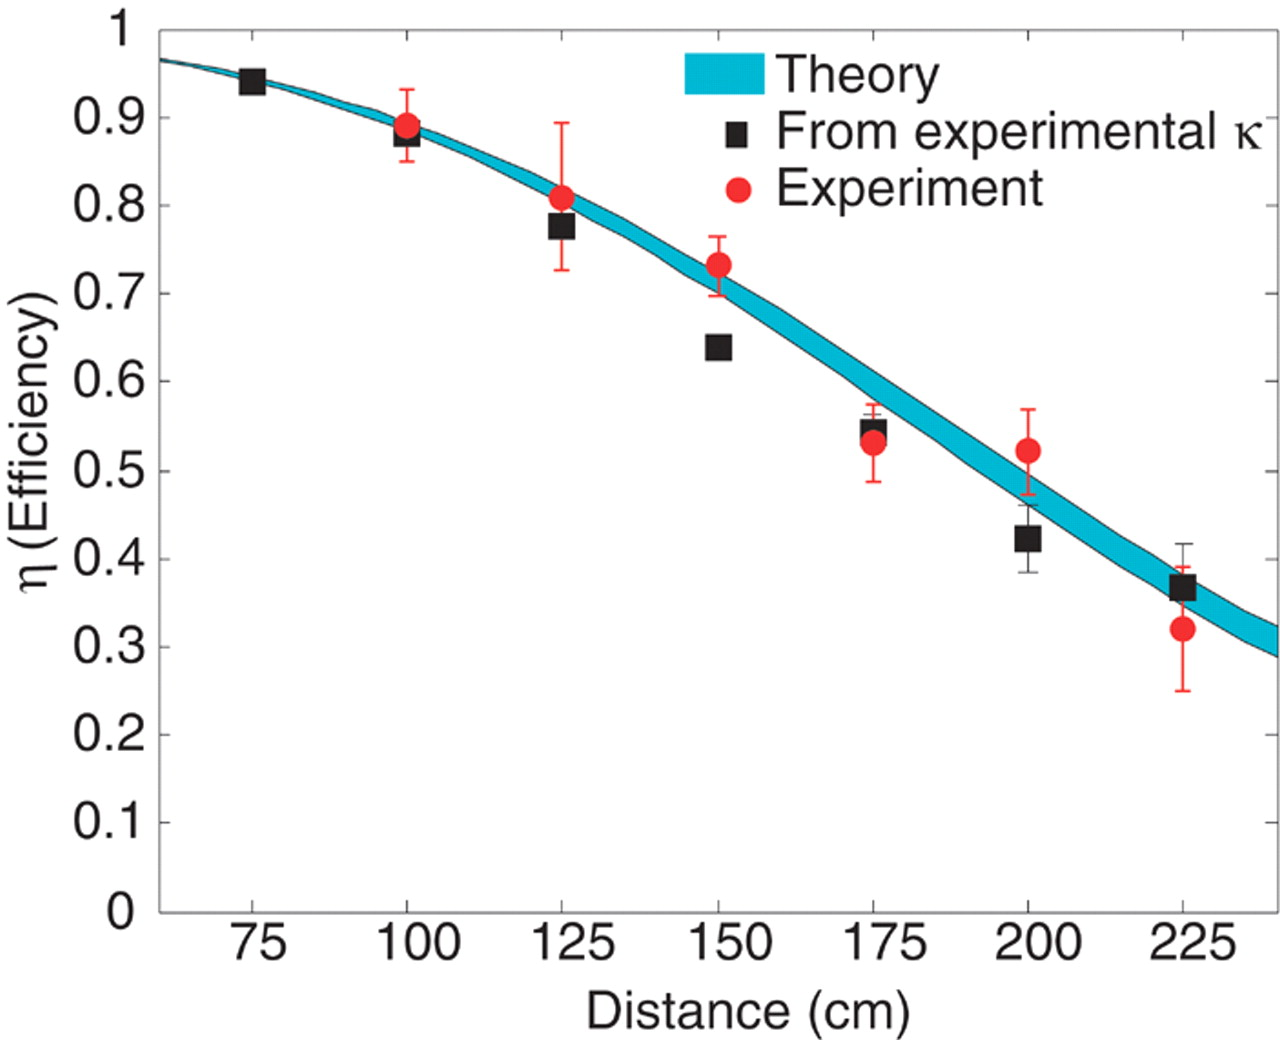
\includegraphics[scale=0.22]{images/Experimental.jpg}
  \caption{A comparison of theoretical and experimental data for the efficiency
  of energy transfer by resonant inductive coupling.
  The data corresponds to a copper wire with a radius of 25cm.
  The blue region and red dots which is the theoretical
  and experimental value respectively is of interest.\cite{StrongCouple}}
  \label{fig:efficiency}
\end{figure}

\section{Application}

There are alternative technologies for wireless energy transfer such as far field methods
and capacitive coupling.
Far field methods involve emission and collection of directional radiation.
This method has a much larger range.
However, the directionality of the emission requires the position of the receiver to
be known ahead of transmission with low tolerance.
Resonant inductive coupling, however, allows for a higher degree of positional freedom.
This is useful in technologies such as smart cards where positioning by consumers
may be imprecise.

\begin{marginfigure}
  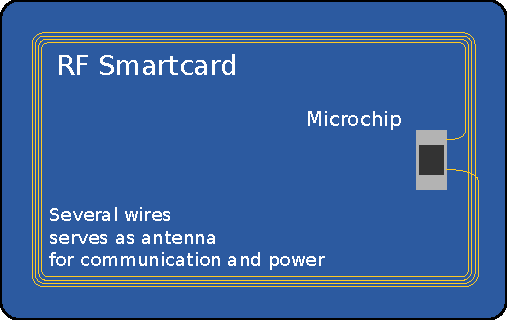
\includegraphics[scale=0.57]{images/smartcard.pdf}
  \caption{One design of smartcards uses a thin copper coil located on the
  edge of the card.
  This coil powers the card when magnetic flux is supplied.
  The coil is also used for communication purposes.\cite{wikiRIC}}
\end{marginfigure}

Widespread adoption of this technology could greatly reduce the need for batteries.
Electrical devices would require less maintenance.
Battery energy often costs
hundreds of times more than mains electricity therefore
the cost of products could be reduced.
In addition, battery disposal is polluting due to chemical waste.
A reduction in battery use would have positive effects on the environment.
\cite{Batteries}

There are concerns about the safety of electromagnetic fields
due to possible interactions with living tissue and jewellery.
Safety is a complicated function of the frequency and power.
Extensive studies have been carried out to find safety limits which
have been tabulated for regulatory purposes.
Therefore, risk can be avoided provided regulations are followed.\cite{IEEE}

\section{Conclusion}

We have shown how the efficiency of energy transfer by electromagnetic
induction can be improved with the addition of resonant circuits.
This occurs as the sensitivity of the resonant circuits results in a feedback
loop.
This alters the magnetic field resulting in more flux flowing through the
receiver than expected, resulting in improved efficiency.
Our discussion then moved to other useful properties of the method including
low directionality, cost, environmental friendliness and safety.
As the technology develops, we speculate that the method will become
increasingly prevalent in the modern world driven by the low maintainability
and cost.




\printbibliography

\end{document}
